\section{CryptoImg}
A paper published in 2009 by Ziad, et al. attempts to implement privacy-preserving image processing using \textit{CryptoImg}, a library for the Open Source Computer Vision Library (OpenCV)~\cite{bradski_opencv_2000} which implements various homomorphic encryption and image processing routines using the Paillier homomorphic cryptosystem~\cite{ziad_cryptoimg:_2016}. The CryptoImg library assumed a client-server model wherein a client requests image processing operations from a server. A client first encrypts a digital image and sends the image securely to a server, which then operates on the encrypted image without revealing its contents. Then the resulting image is sent back to the client, which decrypts the image to recover the desired output.
\begin{figure}[!ht]
    \centering
    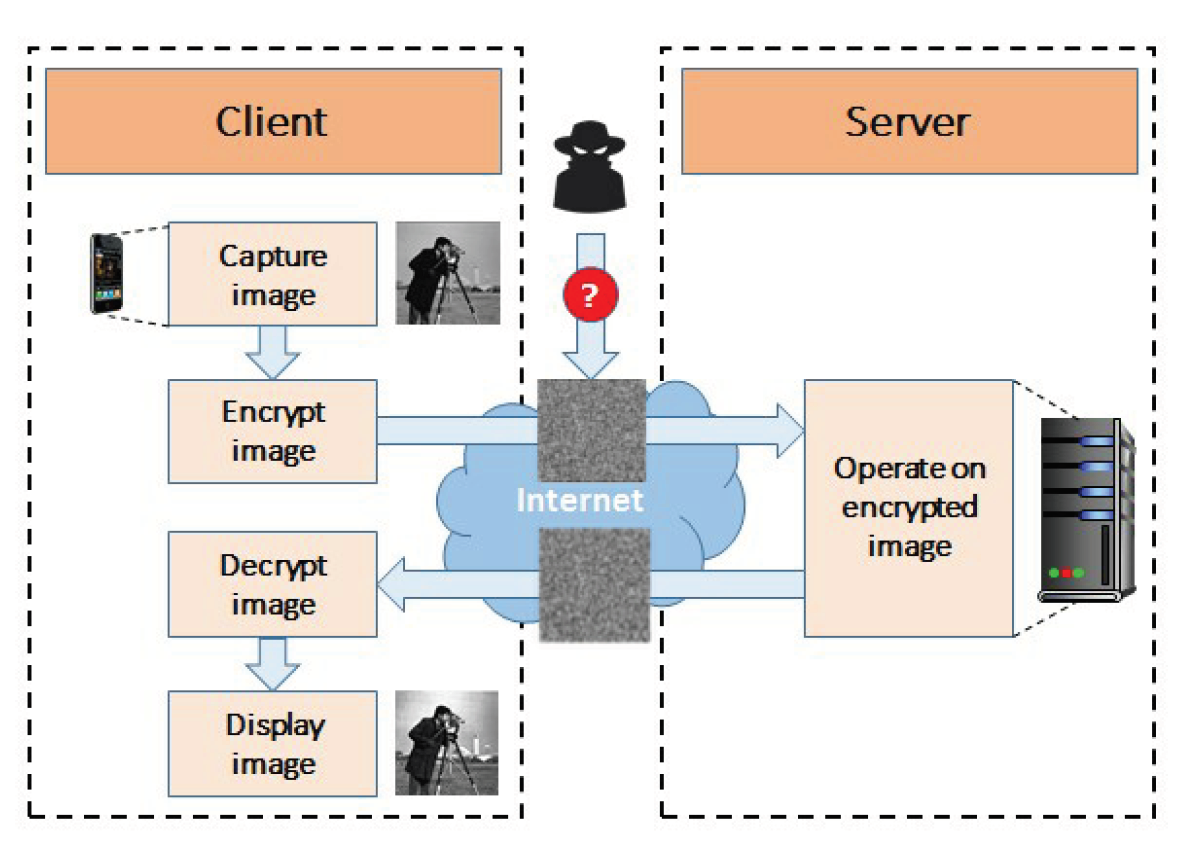
\includegraphics[width=\textwidth,keepaspectratio=true]{Figures/ClientServerModel.png}
    \caption{Client-server architecture used by \textit{CryptoImg} \cite{ziad_cryptoimg:_2016}}
    \label{fig:clientserver}
\end{figure}
The \textit{CryptoImg} library implemented the following:
\begin{enumerate}
	\item Extending the Paillier homomorphic cryptosystem which operate on integer plaintexts so that they can operate on real number plaintexts;
	\item Developing protocols for and implementing the following image processing operations
	\begin{enumerate}
		\item Image negation and brightness adjustment
		\item Spatial filters (for noise reduction, edge detection and sharpening)
		\item Morphological operations
		\item Histogram equalization
	\end{enumerate}
\end{enumerate}
For image negation and spatial filters, the protocols specified by \textit{CryptoImg} allow all image processing operations to be performed on the server. However, due to limitations in the Paillier cryptosystem, the protocols presented for morphological operations and histogram equalization require both the client and the server to perform image processing calculations, although the server performs a significant portion of the processing.

Ziad, et al. also showed experimental results establishing the slow performance of image operations under a homomorphic cryptosystem. For instance, while sharpening and applying a Sobel filter each take less than a second when applied to a $512\times 512$ plaintext image, when applied to an encrypted image, sharpening required at least 238.257 seconds, and applying the Sobel filter required at least 147.567 seconds \cite{ziad_cryptoimg:_2016}.

%%limitations = not considering transcendental function evaluation
%%extension to fully homomorphic cryptosystems
%%combined applications in face detection and recognition

We now discuss several limitations in the \textit{CryptoImg} study which we focus on for our research. First, the \textit{CryptoImg} library was limited in the image intensity transformations it implemented. We propose additional protocols to support more computationally intensive intensity transformations.
Second, the \textit{CryptoImg} library only considered the Paillier cryptosystem. We consider testing the performance of other homomorphic cryptosystems, which differ in their processing time and supported operations.
